% Capitolul 9: Prophet și TBATS
% Prezentare academică de calitate Harvard
% Program de licență, Academia de Studii Economice din București

\documentclass[9pt, aspectratio=169, t]{beamer}

% Asigură încadrarea conținutului pe diapozitive
\setbeamersize{text margin left=8mm, text margin right=8mm}

%=============================================================================
% CONFIGURARE TEMĂ ȘI STIL
%=============================================================================
\usetheme{Madrid}
\usecolortheme{seahorse}

% Paletă de Culori Profesională
\definecolor{MainBlue}{RGB}{26, 58, 110}
\definecolor{AccentBlue}{RGB}{42, 82, 140}
\definecolor{IDAred}{RGB}{220, 53, 69}
\definecolor{DarkGray}{RGB}{51, 51, 51}
\definecolor{MediumGray}{RGB}{128, 128, 128}
\definecolor{LightGray}{RGB}{248, 248, 248}
\definecolor{VeryLightGray}{RGB}{235, 235, 235}
\definecolor{Crimson}{RGB}{220, 53, 69}
\definecolor{Forest}{RGB}{46, 125, 50}
\definecolor{Amber}{RGB}{181, 133, 63}
\definecolor{Orange}{RGB}{230, 126, 34}
\definecolor{HarvardCrimson}{RGB}{165, 28, 48}

\setbeamercolor{palette primary}{bg=MainBlue, fg=white}
\setbeamercolor{palette secondary}{bg=MainBlue!85, fg=white}
\setbeamercolor{palette tertiary}{bg=MainBlue!70, fg=white}
\setbeamercolor{structure}{fg=MainBlue}
\setbeamercolor{title}{fg=MainBlue}
\setbeamercolor{frametitle}{fg=MainBlue, bg=white}
\setbeamercolor{block title}{bg=MainBlue, fg=white}
\setbeamercolor{block body}{bg=VeryLightGray, fg=DarkGray}
\setbeamercolor{block title alerted}{bg=Crimson, fg=white}
\setbeamercolor{block body alerted}{bg=Crimson!8, fg=DarkGray}
\setbeamercolor{block title example}{bg=Forest, fg=white}
\setbeamercolor{block body example}{bg=Forest!8, fg=DarkGray}
\setbeamercolor{item}{fg=MainBlue}

\setbeamertemplate{navigation symbols}{}

\setbeamertemplate{footline}{
    \leavevmode%
    \hbox{%
        \begin{beamercolorbox}[wd=.333333\paperwidth,ht=2.5ex,dp=1ex,center]{author in head/foot}%
            \usebeamerfont{author in head/foot}\insertshortauthor
        \end{beamercolorbox}%
        \begin{beamercolorbox}[wd=.333333\paperwidth,ht=2.5ex,dp=1ex,center]{title in head/foot}%
            \usebeamerfont{title in head/foot}\insertshorttitle
        \end{beamercolorbox}%
        \begin{beamercolorbox}[wd=.333333\paperwidth,ht=2.5ex,dp=1ex,right]{date in head/foot}%
            \usebeamerfont{date in head/foot}\insertshortdate{}\hspace*{2em}
            \insertframenumber{} / \inserttotalframenumber\hspace*{2ex}
        \end{beamercolorbox}}%
    \vskip0pt%
}

%=============================================================================
% PACHETE
%=============================================================================
\usepackage[utf8]{inputenc}
\usepackage[T1]{fontenc}
\usepackage{amsmath, amssymb, amsthm}
\usepackage{mathtools}
\usepackage{bm}
\usepackage{tikz}
\usetikzlibrary{arrows.meta, positioning, shapes, calc, decorations.pathreplacing}
\usepackage{booktabs}
\usepackage{multirow}
\usepackage{array}
\usepackage{graphicx}
\usepackage{hyperref}
\usepackage{colortbl}
\hypersetup{colorlinks=false, pdfborder={0 0 0}}
\graphicspath{{../logos/}{../charts/}}

%=============================================================================
% MEDII PENTRU TEOREME
%=============================================================================
\theoremstyle{definition}
\setbeamertemplate{theorems}[numbered]
\newtheorem{defn}{Definiție}
\newtheorem{thm}{Teoremă}
\newtheorem{prop}{Propoziție}
\newtheorem{rmk}{Observație}

%=============================================================================
% COMENZI PERSONALIZATE
%=============================================================================
\newcommand{\E}{\mathbb{E}}
\newcommand{\Var}{\text{Var}}
\newcommand{\Cov}{\text{Cov}}
\newcommand{\Corr}{\text{Corr}}
\newcommand{\R}{\mathbb{R}}
\newcommand{\N}{\mathbb{N}}
\newcommand{\Z}{\mathbb{Z}}
\newcommand{\RMSE}{\text{RMSE}}
\newcommand{\MAE}{\text{MAE}}
\newcommand{\MAPE}{\text{MAPE}}

%=============================================================================
% INFORMAȚII TITLU
%=============================================================================
\title[Capitolul 9: Prophet \& TBATS]{Capitolul 9: Prophet și TBATS}
\subtitle{Program de licență, Facultatea de Cibernetică, Statistică și Informatică Economică, Academia de Studii Economice din București}
\author[Prof. dr. Daniel Traian Pele]{Prof. dr. Daniel Traian Pele\\[0.2cm]\footnotesize\texttt{danpele@ase.ro}}
\institute{Academia de Studii Economice din București}
\date{An Universitar 2025--2026}

\begin{document}

%=============================================================================
% DIAPOZITIV TITLU
%=============================================================================
\begin{frame}[plain]
    \begin{tikzpicture}[remember picture, overlay]
        \fill[IDAred] (current page.north west) rectangle ([yshift=-0.15cm]current page.north east);
        \node[anchor=north west] at ([xshift=0.5cm, yshift=-0.3cm]current page.north west) {
            \href{https://www.ase.ro}{\includegraphics[height=1.1cm]{ase_logo.png}}
        };
        \node[anchor=north] at ([yshift=-0.3cm]current page.north) {
            \href{https://ai4efin.ase.ro}{\includegraphics[height=1.1cm]{ai4efin_logo.png}}
        };
        \node[anchor=north east] at ([xshift=-0.5cm, yshift=-0.3cm]current page.north east) {
            \href{https://www.digital-finance-msca.com}{\includegraphics[height=1.1cm]{msca_logo.png}}
        };
    \end{tikzpicture}
    \vfill
    \begin{center}
        {\Large\textcolor{MediumGray}{Analiza și Prognoză Seriilor de Timp}}\\[0.3cm]
        {\Huge\textbf{\textcolor{MainBlue}{Capitolul 9: Prophet și TBATS}}}\\[0.5cm]
        {\Large\textcolor{IDAred}{Modele Moderne pentru Sezonalități Multiple}}
    \end{center}
    \vfill

    \begin{tikzpicture}[remember picture, overlay]
        \fill[IDAred] (current page.south west) rectangle ([yshift=0.15cm]current page.south east);
        \node[anchor=south west] at ([xshift=0.5cm, yshift=0.8cm]current page.south west) {
            \href{https://theida.net}{\includegraphics[height=0.9cm]{ida_logo.png}}
        };
        \node[anchor=south] at ([xshift=-3cm, yshift=0.8cm]current page.south) {
            \href{https://blockchain-research-center.com}{\includegraphics[height=0.9cm]{brc_logo.png}}
        };
        \node[anchor=south] at ([yshift=0.8cm]current page.south) {
            \href{https://quantinar.com}{\includegraphics[height=0.9cm]{qr_logo.png}}
        };
        \node[anchor=south] at ([xshift=3cm, yshift=0.8cm]current page.south) {
            \href{https://quantlet.com}{\includegraphics[height=0.9cm]{ql_logo.png}}
        };
        \node[anchor=south east] at ([xshift=-0.5cm, yshift=0.8cm]current page.south east) {
            \href{https://ipe.ro/new}{\includegraphics[height=0.9cm]{acad_logo.png}}
        };
    \end{tikzpicture}
\end{frame}

%=============================================================================
% OUTLINE
%=============================================================================
\begin{frame}{Cuprins}
    \tableofcontents
\end{frame}

%=============================================================================
% SECTION 1: MOTIVATION
%=============================================================================
\section{Sezonalități Multiple}

\begin{frame}{Problema: Tipare Sezoniere Complexe}
    \begin{block}{Exemple din Lumea Reală}
        \begin{itemize}
            \item \textbf{Cerere de electricitate pe oră}: Tipare zilnice + săptămânale + anuale
            \item \textbf{Trafic web}: Zilnic + săptămânal + efecte de sărbători
            \item \textbf{Vânzări retail}: Săptămânal + lunar + anual + sărbători
            \item \textbf{Volum call center}: Pe oră + zilnic + săptămânal
        \end{itemize}
    \end{block}

    \vspace{0.3cm}

    \begin{alertblock}{Limitarea SARIMA}
        SARIMA$(p,d,q)(P,D,Q)_s$ standard gestionează doar \textbf{o singură} perioadă sezonieră $s$.

        \vspace{0.2cm}
        Pentru date orare cu tipare zilnice ȘI săptămânale, avem nevoie de $s_1 = 24$ și $s_2 = 168$.
    \end{alertblock}
\end{frame}

\begin{frame}{Soluții pentru Sezonalități Multiple}
    \begin{columns}[T]
        \column{0.5\textwidth}
        \begin{block}{Abordări Tradiționale}
            \begin{itemize}
                \item \textbf{Termeni Fourier}: Adăugare regresori sin/cos
                \item \textbf{Variabile dummy}: Mulți parametri
                \item \textbf{Modele nested}: Specificare complexă
            \end{itemize}
        \end{block}

        \column{0.5\textwidth}
        \begin{exampleblock}{Abordări Moderne}
            \begin{itemize}
                \item \textbf{TBATS}: Automat, gestionează multe perioade
                \item \textbf{Prophet}: Flexibil, interpretabil
                \item \textbf{Metode neurale}: Deep learning
            \end{itemize}
        \end{exampleblock}
    \end{columns}

    \vspace{0.5cm}

    \begin{center}
        \begin{tabular}{lcc}
            \toprule
            \textbf{Metodă} & \textbf{Nr. Max Sezonalități} & \textbf{Interpretabil} \\
            \midrule
            SARIMA & 1 & Da \\
            Fourier + ARIMA & Multiple & Moderat \\
            TBATS & Multiple & Moderat \\
            Prophet & Multiple & Da \\
            \bottomrule
        \end{tabular}
    \end{center}
\end{frame}

\begin{frame}{Exemplu: Date Orare cu Sezonalități Multiple}
    \begin{center}
        \includegraphics[width=0.95\textwidth, height=0.70\textheight, keepaspectratio]{ch9_multiple_seasonality.pdf}
    \end{center}
\end{frame}

\begin{frame}{Exemplu Real: Cerere de Electricitate}
    \begin{center}
        \includegraphics[width=0.95\textwidth, height=0.70\textheight, keepaspectratio]{ch9_electricity_demand.pdf}
    \end{center}
\end{frame}

\begin{frame}{Exemplu Real: Vânzări Retail cu Sărbători}
    \begin{center}
        \includegraphics[width=0.95\textwidth, height=0.70\textheight, keepaspectratio]{ch9_retail_sales.pdf}
    \end{center}
\end{frame}

%=============================================================================
% SECTION 2: TBATS
%=============================================================================
\section{Modelul TBATS}

\begin{frame}{TBATS: Ce Înseamnă?}
    \begin{block}{Componentele TBATS}
        \begin{description}
            \item[T] Sezonalitate \textbf{Trigonometrică} folosind termeni Fourier
            \item[B] Transformare \textbf{Box-Cox} pentru stabilizarea varianței
            \item[A] Erori \textbf{ARMA} pentru autocorelația reziduală
            \item[T] Componentă de \textbf{Trend} (posibil amortizat)
            \item[S] Componente \textbf{Sezoniere} (multiple permise)
        \end{description}
    \end{block}

    \vspace{0.3cm}

    \begin{exampleblock}{Inovația Cheie}
        TBATS folosește \textbf{reprezentare trigonometrică} pentru sezonalitate:
        \[
        s_t^{(i)} = \sum_{j=1}^{k_i} \left[ s_j^{(i)} \cos\left(\frac{2\pi j t}{m_i}\right) + s_j^{*(i)} \sin\left(\frac{2\pi j t}{m_i}\right) \right]
        \]
        unde $m_i$ este perioadă sezonieră $i$ și $k_i$ este numărul de armonici.
    \end{exampleblock}
\end{frame}

\begin{frame}{Structura Modelului TBATS}
    \begin{block}{Specificația Completă a Modelului}
        \begin{align}
            y_t^{(\omega)} &= \ell_{t-1} + \phi b_{t-1} + \sum_{i=1}^{T} s_{t-m_i}^{(i)} + d_t \\[0.3cm]
            \ell_t &= \ell_{t-1} + \phi b_{t-1} + \alpha d_t \\[0.2cm]
            b_t &= \phi b_{t-1} + \beta d_t \\[0.2cm]
            d_t &= \sum_{i=1}^{p} \varphi_i d_{t-i} + \sum_{j=1}^{q} \theta_j \varepsilon_{t-j} + \varepsilon_t
        \end{align}
    \end{block}

    \vspace{0.1cm}

    {\footnotesize
    Unde:
    \begin{itemize}
        \item $y_t^{(\omega)}$ este seria transformată Box-Cox (dacă $\omega \neq 1$)
        \item $\ell_t$ este nivelul local, $b_t$ este trendul cu amortizare $\phi$
        \item $s_t^{(i)}$ sunt $T$ componente sezoniere cu perioade $m_1, \ldots, m_T$
        \item $d_t$ este procesul de eroare ARMA$(p,q)$
    \end{itemize}
    }
\end{frame}

\begin{frame}{TBATS: Sezonalitate Trigonometrică}
    \begin{block}{De Ce Termeni Fourier/Trigonometrici?}
        \begin{enumerate}
            \item \textbf{Simplu}: Mai puțini parametri decât variabilele dummy
            \item \textbf{Neted}: Captează natural tiparele sezoniere netede
            \item \textbf{Flexibil}: Numărul de armonici $k$ controlează complexitatea
            \item \textbf{Perioade non-întregi}: Poate gestiona $s = 365.25$ pentru date zilnice
        \end{enumerate}
    \end{block}

    \vspace{0.3cm}

    \begin{columns}[T]
        \column{0.5\textwidth}
        \begin{exampleblock}{$k$ mic (puține armonici)}
            \begin{itemize}
                \item Tipar neted
                \item Mai puțini parametri
                \item Poate rata vârfuri abrupte
            \end{itemize}
        \end{exampleblock}

        \column{0.5\textwidth}
        \begin{alertblock}{$k$ mare (multe armonici)}
            \begin{itemize}
                \item Poate capta orice tipar
                \item Mai mulți parametri
                \item Risc de supraajustare
            \end{itemize}
        \end{alertblock}
    \end{columns}
\end{frame}

\begin{frame}{Aproximarea Fourier a Sezonalității}
    \begin{center}
        \includegraphics[width=0.95\textwidth, height=0.70\textheight, keepaspectratio]{ch9_fourier_approximation.pdf}
    \end{center}
\end{frame}

\begin{frame}{TBATS în Practică}
    \begin{block}{Implementare Python}
        Pachetul \texttt{tbats} oferă selecție automată a modelului:
        \begin{itemize}
            \item Selectează automat parametrul Box-Cox $\omega$
            \item Alege numărul de armonici $k_i$ pentru fiecare perioadă sezonieră
            \item Selectează ordinele ARMA $(p,q)$
            \item Testează trend amortizat vs neamortizat
        \end{itemize}
    \end{block}

    \vspace{0.3cm}

    \begin{exampleblock}{Exemplu de Cod}
        \small
        \texttt{from tbats import TBATS}\\
        \texttt{eștimator = TBATS(seasonal\_periods=[7, 365.25])}\\
        \texttt{model = eștimator.fit(y)}\\
        \texttt{forecast = model.forecast(steps=30)}
    \end{exampleblock}

    \vspace{0.2cm}

    {\small \textbf{Notă}: BATS este versiunea mai simplă fără termeni trigonometrici (folosește stări sezoniere tradiționale).}
\end{frame}

\begin{frame}{TBATS: Avantaje și Limitări}
    \begin{columns}[T]
        \column{0.5\textwidth}
        \begin{exampleblock}{Avantaje}
            \begin{itemize}
                \item Gestionează \textbf{multiple} perioade sezoniere
                \item Selecție \textbf{automată} a modelului
                \item Gestionează perioade \textbf{non-întregi} (365.25)
                \item \textbf{Box-Cox} pentru heteroscedasticitate
                \item Bun pentru date de \textbf{frecvență înaltă}
            \end{itemize}
        \end{exampleblock}

        \column{0.5\textwidth}
        \begin{alertblock}{Limitări}
            \begin{itemize}
                \item \textbf{Intensiv computațional}
                \item Fără \textbf{regresori externi}
                \item Mai puțin \textbf{interpretabil} decât Prophet
                \item Poate fi \textbf{lent} pentru serii foarte lungi
                \item Necesită \textbf{suficiente date} per sezon
            \end{itemize}
        \end{alertblock}
    \end{columns}
\end{frame}

\begin{frame}{Exemplu Descompunere TBATS}
    \begin{center}
        \includegraphics[width=0.95\textwidth, height=0.70\textheight, keepaspectratio]{ch9_tbats_decomposition.pdf}
    \end{center}
\end{frame}

%=============================================================================
% SECTION 3: PROPHET
%=============================================================================
\section{Facebook Prophet}

\begin{frame}{Prophet: Prezentare Generală}
    \begin{block}{Ce este Prophet?}
        Prophet este o procedură de prognoză dezvoltată de Facebook (Meta) în 2017.

        \vspace{0.2cm}

        Proiectat pentru \textbf{serii de timp de business} cu:
        \begin{itemize}
            \item Efecte sezoniere puternice (zilnice, săptămânale, anuale)
            \item Efecte de sărbători
            \item Schimbări de trend (changepoints)
            \item Date lipsă și outlieri
        \end{itemize}
    \end{block}

    \vspace{0.3cm}

    \begin{exampleblock}{Filosofia Cheie}
        \begin{center}
            \textit{``Analyst-in-the-loop'' forecasting}
        \end{center}
        Prophet este proiectat pentru a fi ajustat de analiști cu cunoștințe de domeniu, dar care nu sunt neapărat experți în serii de timp.
    \end{exampleblock}
\end{frame}

\begin{frame}{Structura Modelului Prophet}
    \begin{block}{Abordare prin Descompunere}
        Prophet folosește o \textbf{descompunere aditivă}:
        \[
        y(t) = g(t) + s(t) + h(t) + \varepsilon_t
        \]
    \end{block}

    \vspace{0.3cm}

    \begin{columns}[T]
        \column{0.33\textwidth}
        \begin{block}{$g(t)$: Trend}
            \begin{itemize}
                \item Liniar sau logistic
                \item Changepoints automate
                \item Saturație de creștere
            \end{itemize}
        \end{block}

        \column{0.33\textwidth}
        \begin{block}{$s(t)$: Sezonalitate}
            \begin{itemize}
                \item Serii Fourier
                \item Perioade multiple
                \item Sezonalitate custom
            \end{itemize}
        \end{block}

        \column{0.33\textwidth}
        \begin{block}{$h(t)$: Sărbători}
            \begin{itemize}
                \item Sărbători pe țară
                \item Evenimente custom
                \item Efecte de fereastră
            \end{itemize}
        \end{block}
    \end{columns}
\end{frame}

\begin{frame}{Prophet: Componenta de Trend}
    \begin{block}{Trend Liniar cu Changepoints}
        \[
        g(t) = (k + \bm{a}(t)^T \bm{\delta}) \cdot t + (m + \bm{a}(t)^T \bm{\gamma})
        \]
        unde:
        \begin{itemize}
            \item $k$ este rata de creștere de bază
            \item $\bm{\delta}$ este un vector de ajustări de rată la changepoints
            \item $\bm{a}(t)$ indică ce changepoints sunt active la momentul $t$
            \item $m$ este offset-ul, $\bm{\gamma}$ asigură continuitatea
        \end{itemize}
    \end{block}

    \vspace{0.3cm}

    \begin{exampleblock}{Creștere Logistică (pentru trenduri cu saturație)}
        \[
        g(t) = \frac{C(t)}{1 + \exp(-(k + \bm{a}(t)^T \bm{\delta})(t - (m + \bm{a}(t)^T \bm{\gamma})))}
        \]
        unde $C(t)$ este capacitatea maximă (posibil variabilă în timp).
    \end{exampleblock}
\end{frame}

\begin{frame}{Prophet: Componenta de Sezonalitate}
    \begin{block}{Reprezentare prin Serii Fourier}
        Pentru o perioadă sezonieră $P$, Prophet folosește:
        \[
        s(t) = \sum_{n=1}^{N} \left[ a_n \cos\left(\frac{2\pi n t}{P}\right) + b_n \sin\left(\frac{2\pi n t}{P}\right) \right]
        \]
    \end{block}

    \vspace{0.3cm}

    \begin{exampleblock}{Setări Implicite}
        \begin{center}
        \begin{tabular}{lcc}
            \toprule
            \textbf{Sezonalitate} & \textbf{Perioadă} & \textbf{Ordin Fourier} \\
            \midrule
            Anuală & 365.25 zile & 10 \\
            Săptămânală & 7 zile & 3 \\
            Zilnică & 1 zi & 4 \\
            \bottomrule
        \end{tabular}
        \end{center}
    \end{exampleblock}

    \vspace{0.2cm}

    {\small Ordin Fourier $N$ mai mare = mai multă flexibilitate (poate ajusta tipare mai complexe) dar risc mai mare de supraajustare.}
\end{frame}

\begin{frame}{Descompunerea Componentelor Prophet}
    \begin{center}
        \includegraphics[width=0.95\textwidth, height=0.70\textheight, keepaspectratio]{ch9_prophet_components.pdf}
    \end{center}
\end{frame}

\begin{frame}{Detectarea Changepoints în Trend}
    \begin{center}
        \includegraphics[width=0.95\textwidth, height=0.70\textheight, keepaspectratio]{ch9_changepoint_detection.pdf}
    \end{center}
\end{frame}

\begin{frame}{Prophet: Efecte de Sărbători}
    \begin{block}{Modelul de Sărbători}
        \[
        h(t) = Z(t) \cdot \bm{\kappa}
        \]
        unde $Z(t)$ este o matrice indicător pentru sărbători și $\bm{\kappa}$ sunt efectele sărbătorilor.
    \end{block}

    \vspace{0.3cm}

    \begin{exampleblock}{Caracteristici}
        \begin{itemize}
            \item \textbf{Sărbători integrate}: 60+ țări suportate
            \item \textbf{Sărbători custom}: Adăugați propriile evenimente (Black Friday, evenimente companie)
            \item \textbf{Efecte de fereastră}: Sărbătorile pot afecta zilele înainte/după
            \item \textbf{Prior scale}: Controlează regularizarea efectelor de sărbătoare
        \end{itemize}
    \end{exampleblock}

    \vspace{0.3cm}

    \begin{block}{Exemplu de Cod}
        \small
        \texttt{holidays = pd.DataFrame(\{'holiday': 'black\_friday', ....\})}\\
        \texttt{model = Prophet(holidays=holidays)}
    \end{block}
\end{frame}

\begin{frame}{Prophet în Practică}
    \begin{block}{Utilizare de Bază}
        \small
        \texttt{from prophet import Prophet}\\
        \texttt{import pandas as pd}\\[0.2cm]
        \texttt{\# Datele trebuie să aibă coloane 'ds' (dată) și 'y' (valoare)}\\
        \texttt{df = pd.DataFrame(\{'ds': dates, 'y': values\})}\\[0.2cm]
        \texttt{model = Prophet()}\\
        \texttt{model.fit(df)}\\[0.2cm]
        \texttt{future = model.make\_future\_dataframe(periods=365)}\\
        \texttt{forecast = model.predict(future)}
    \end{block}

    \vspace{0.3cm}

    \begin{exampleblock}{Adăugare Sezonalitate Custom}
        \small
        \texttt{model = Prophet(weekly\_seasonality=False)}\\
        \texttt{model.add\_seasonality(name='monthly', period=30.5, fourier\_order=5)}\\
        \texttt{model.add\_seasonality(name='quarterly', period=91.25, fourier\_order=3)}
    \end{exampleblock}
\end{frame}

\begin{frame}{Prophet: Cuantificarea Incertitudinii}
    \begin{block}{Trei Surse de Incertitudine}
        \begin{enumerate}
            \item \textbf{Incertitudine de trend}: Changepoints viitoare sunt incerte
            \item \textbf{Incertitudine de sezonalitate}: Incertitudine în estimarea parametrilor
            \item \textbf{Zgomot de observație}: Aleatorietate inerentă
        \end{enumerate}
    \end{block}

    \vspace{0.3cm}

    \begin{columns}[T]
        \column{0.6\textwidth}
        \begin{exampleblock}{Intervale de Predicție}
            Prophet oferă:
            \begin{itemize}
                \item Prognoză punctuală: \texttt{yhat}
                \item Limita inferioară: \texttt{yhat\_lower}
                \item Limita superioară: \texttt{yhat\_upper}
            \end{itemize}

            \vspace{0.2cm}

            Implicit este interval de 80\%.\\
            Schimbați cu \texttt{interval\_width=0.95}
        \end{exampleblock}

        \column{0.4\textwidth}
        \begin{alertblock}{Notă}
            Incertitudinea crește cu orizontul de prognoză, în special pentru incertitudinea de trend.
        \end{alertblock}
    \end{columns}
\end{frame}

\begin{frame}{Prophet: Parametri de Ajustare}
    \begin{block}{Parametri Cheie}
        \begin{center}
        \small
        \begin{tabular}{p{4cm}p{8cm}}
            \toprule
            \textbf{Parametru} & \textbf{Efect} \\
            \midrule
            \texttt{changepoint\_prior\_scale} & Flexibilitate trend (implicit: 0.05) \\
            \texttt{seasonality\_prior\_scale} & Flexibilitate sezonalitate (implicit: 10) \\
            \texttt{holidays\_prior\_scale} & Mărime efect sărbători (implicit: 10) \\
            \texttt{seasonality\_mode} & 'additive' sau 'multiplicative' \\
            \texttt{changepoint\_range} & Porțiune din istoric pentru changepoints \\
            \bottomrule
        \end{tabular}
        \end{center}
    \end{block}

    \vspace{0.3cm}

    \begin{exampleblock}{Sfaturi Practice}
        \begin{itemize}
            \item \textbf{Supraajustare pe trend?} Micșorați \texttt{changepoint\_prior\_scale}
            \item \textbf{Subajustare pe sezonalitate?} Măriți \texttt{seasonality\_prior\_scale}
            \item \textbf{Amplitudinea sezonieră variază?} Folosiți \texttt{seasonality\_mode='multiplicative'}
        \end{itemize}
    \end{exampleblock}
\end{frame}

\begin{frame}{Prophet: Avantaje și Limitări}
    \begin{columns}[T]
        \column{0.5\textwidth}
        \begin{exampleblock}{Avantaje}
            \begin{itemize}
                \item \textbf{Ușor de folosit}: Ajustare minimă necesară
                \item \textbf{Interpretabil}: Descompunere clară
                \item \textbf{Gestionează date lipsă} bine
                \item \textbf{Efecte sărbători} integrate
                \item \textbf{Sezonalități multiple}
                \item \textbf{Regresori externi} suportați
                \item \textbf{Ajustare rapidă}
            \end{itemize}
        \end{exampleblock}

        \column{0.5\textwidth}
        \begin{alertblock}{Limitări}
            \begin{itemize}
                \item \textbf{Nu bazat pe ARIMA}: Fără modelare autocorelație
                \item \textbf{Focus pe date zilnice}: Mai puțin potrivit pentru frecvență foarte înaltă
                \item \textbf{Ipoteze de trend}: Liniar/logistic poate să nu se potrivească
                \item \textbf{Fără CV integrat}: Trebuie implementat manual
                \item \textbf{Risc supraajustare} cu multe sezonalități
            \end{itemize}
        \end{alertblock}
    \end{columns}
\end{frame}

\begin{frame}{Sezonalitate Aditivă vs Multiplicativă}
    \begin{center}
        \includegraphics[width=0.95\textwidth, height=0.70\textheight, keepaspectratio]{ch9_additive_vs_multiplicative.pdf}
    \end{center}
\end{frame}

%=============================================================================
% SECTION 4: COMPARISON
%=============================================================================
\section{Comparație și Ghid de Selecție}

\begin{frame}{TBATS vs Prophet: Comparație Directă}
    \begin{center}
    \small
    \begin{tabular}{p{4cm}p{4.5cm}p{4.5cm}}
        \toprule
        \textbf{Caracteristică} & \textbf{TBATS} & \textbf{Prophet} \\
        \midrule
        Sezonalități multiple & Da (automat) & Da (manual sau auto) \\
        Efecte sărbători & Nu & Da (integrat) \\
        Regresori externi & Nu & Da \\
        Changepoints trend & Nu (neted) & Da (automat) \\
        Date lipsă & Necesită interpolare & Gestionează nativ \\
        Interpretabilitate & Moderată & Înaltă \\
        Viteză calcul & Lent & Rapid \\
        Date frecvență înaltă & Bun & Moderat \\
        Perioade non-întregi & Da (ex: 365.25) & Da \\
        Intervale incertitudine & Da & Da \\
        \bottomrule
    \end{tabular}
    \end{center}
\end{frame}

\begin{frame}{Comparație Prophet vs TBATS: Prognoze}
    \begin{center}
        \includegraphics[width=0.95\textwidth, height=0.70\textheight, keepaspectratio]{ch9_prophet_vs_tbats.pdf}
    \end{center}
\end{frame}

\begin{frame}{Când să Folosim Fiecare Model}
    \begin{columns}[T]
        \column{0.5\textwidth}
        \begin{block}{Folosiți TBATS când:}
            \begin{itemize}
                \item Date de frecvență înaltă (orare, sub-zilnice)
                \item Multiple perioade sezoniere complexe
                \item Nu sunt necesari regresori externi
                \item Se preferă selecție automată a modelului
                \item Se dorește framework tradițional state-space
            \end{itemize}
        \end{block}

        \column{0.5\textwidth}
        \begin{block}{Folosiți Prophet când:}
            \begin{itemize}
                \item Prognoză de business (zilnic/săptămânal)
                \item Efectele sărbătorilor sunt importante
                \item Trendul are rupturi structurale
                \item Sunt prezente date lipsă
                \item Interpretabilitatea este cheie
                \item Sunt disponibili regresori externi
            \end{itemize}
        \end{block}
    \end{columns}

    \vspace{0.5cm}

    \begin{exampleblock}{Ghid General}
        \begin{center}
            \textbf{Prophet} pentru aplicații de business cu date zilnice\\
            \textbf{TBATS} pentru aplicații tehnice cu date de frecvență înaltă
        \end{center}
    \end{exampleblock}
\end{frame}

\begin{frame}{Ghid Selecție Model}
    \begin{center}
        \includegraphics[width=0.90\textwidth, height=0.60\textheight, keepaspectratio]{ch9_model_selection_guide.pdf}
    \end{center}
\end{frame}

\begin{frame}{Diagramă de Decizie}
    \begin{center}
    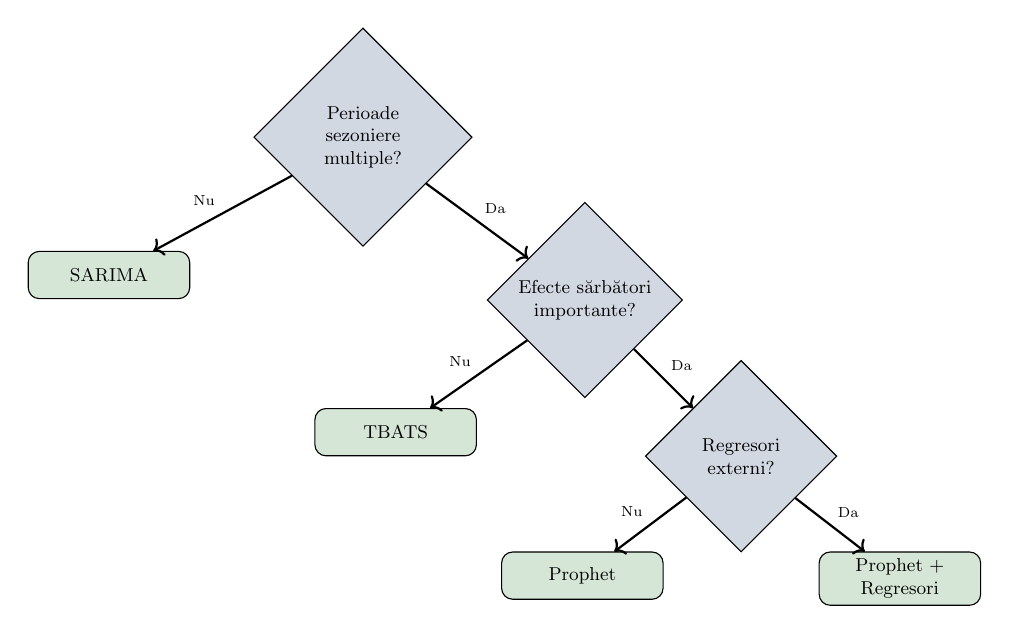
\begin{tikzpicture}[
        scale=0.75, transform shape,
        node distance=1.2cm,
        decision/.style={diamond, draw, fill=MainBlue!20, text width=2.5cm, text centered, inner sep=1pt, font=\small},
        block/.style={rectangle, draw, fill=Forest!20, text width=2.5cm, text centered, rounded corners, minimum height=0.8cm, font=\small},
        line/.style={draw, ->, thick}
    ]
        \node [decision] (q1) {Perioade sezoniere multiple?};
        \node [block, below left=1cm and 2cm of q1] (sarima) {SARIMA};
        \node [decision, below right=1cm and 2cm of q1] (q2) {Efecte sărbători importante?};
        \node [block, below left=1cm and 1cm of q2] (tbats) {TBATS};
        \node [decision, below right=1cm and 1cm of q2] (q3) {Regresori externi?};
        \node [block, below left=0.8cm and 0.5cm of q3] (prophet1) {Prophet};
        \node [block, below right=0.8cm and 0.5cm of q3] (prophet2) {Prophet + Regresori};

        \path [line] (q1) -- node[above left, font=\scriptsize] {Nu} (sarima);
        \path [line] (q1) -- node[above right, font=\scriptsize] {Da} (q2);
        \path [line] (q2) -- node[above left, font=\scriptsize] {Nu} (tbats);
        \path [line] (q2) -- node[above right, font=\scriptsize] {Da} (q3);
        \path [line] (q3) -- node[above left, font=\scriptsize] {Nu} (prophet1);
        \path [line] (q3) -- node[above right, font=\scriptsize] {Da} (prophet2);
    \end{tikzpicture}
    \end{center}
\end{frame}

%=============================================================================
% SECTION 5: PRACTICAL EXAMPLE
%=============================================================================
\section{Studiu de Caz}

\begin{frame}{Studiu de Caz: Prognoză Cererii de Energie}
    \begin{block}{Problema}
        Prognozăți cererea de electricitate pe oră cu:
        \begin{itemize}
            \item \textbf{Tipar zilnic}: Vârf la prânz și seara
            \item \textbf{Tipar săptămânal}: Mai scăzut în weekend
            \item \textbf{Tipar anual}: Mai mare vara (AC) și iarna (încălzire)
            \item \textbf{Efecte sărbători}: Cerere mai mică în sărbători
        \end{itemize}
    \end{block}

    \vspace{0.3cm}

    \begin{exampleblock}{Abordare}
        \begin{enumerate}
            \item Încercați TBATS cu perioade [24, 168, 8766]
            \item Încercați Prophet cu sezonalitate zilnică, săptămânală, anuală + sărbători
            \item Comparați folosind cross-validation
        \end{enumerate}
    \end{exampleblock}
\end{frame}

\begin{frame}{Studiu de Caz: Interpretarea Rezultatelor}
    \begin{block}{Metrici de Evaluare}
        \begin{itemize}
            \item \textbf{MAPE}: Mean Absolute Percentage Error
            \item \textbf{RMSE}: Root Mean Square Error
            \item \textbf{Acoperire}: \% din valori reale în intervalul de predicție
        \end{itemize}
    \end{block}

    \vspace{0.3cm}

    \begin{exampleblock}{Rezultate Tipice}
        \begin{center}
        \begin{tabular}{lccc}
            \toprule
            \textbf{Model} & \textbf{MAPE} & \textbf{RMSE} & \textbf{Acoperire} \\
            \midrule
            SARIMA (doar zilnic) & 8.5\% & 450 MW & 75\% \\
            TBATS & 4.2\% & 220 MW & 82\% \\
            Prophet & 4.8\% & 250 MW & 85\% \\
            Prophet + sărbători & 3.9\% & 200 MW & 88\% \\
            \bottomrule
        \end{tabular}
        \end{center}
    \end{exampleblock}

    {\small Modelele cu sezonalități multiple depășesc semnificativ SARIMA cu o singură sezonalitate.}
\end{frame}

%=============================================================================
% SECTION 6: SUMMARY
%=============================================================================
\section{Sumar}

\begin{frame}{Concluzii Cheie}
    \begin{block}{Sezonalități Multiple}
        \begin{itemize}
            \item Datele din lumea reală au adesea tipare sezoniere multiple
            \item SARIMA standard gestionează doar o perioadă sezonieră
            \item TBATS și Prophet sunt proiectate pentru această provocare
        \end{itemize}
    \end{block}

    \vspace{0.3cm}

    \begin{exampleblock}{Selecția Modelului}
        \begin{itemize}
            \item \textbf{TBATS}: Automat, gestionează frecvență înaltă, fără regresori externi
            \item \textbf{Prophet}: Interpretabil, efecte sărbători, regresori externi
            \item Ambele folosesc termeni Fourier pentru reprezentare eficientă a sezonalității
        \end{itemize}
    \end{exampleblock}

    \vspace{0.3cm}

    \begin{alertblock}{De Reținut}
        Validați întotdeauna cu cross-validation adecvat pentru serii de timp!
    \end{alertblock}
\end{frame}

\begin{frame}{Întrebări?}
    \begin{center}
        \Large\textcolor{MainBlue}{Întrebări?}

        \vspace{1cm}

        \normalsize
        \textbf{Pași Următori:}
        \begin{itemize}
            \item Exersați cu notebook-ul Jupyter
            \item Încercați Prophet pe propriile date
            \item Explorați NeuralProphet pentru extensia deep learning
        \end{itemize}
    \end{center}
\end{frame}

\end{document}
